\documentclass{article}

\usepackage{tikz}
\usetikzlibrary{arrows}

\begin{document}

\begin{center}
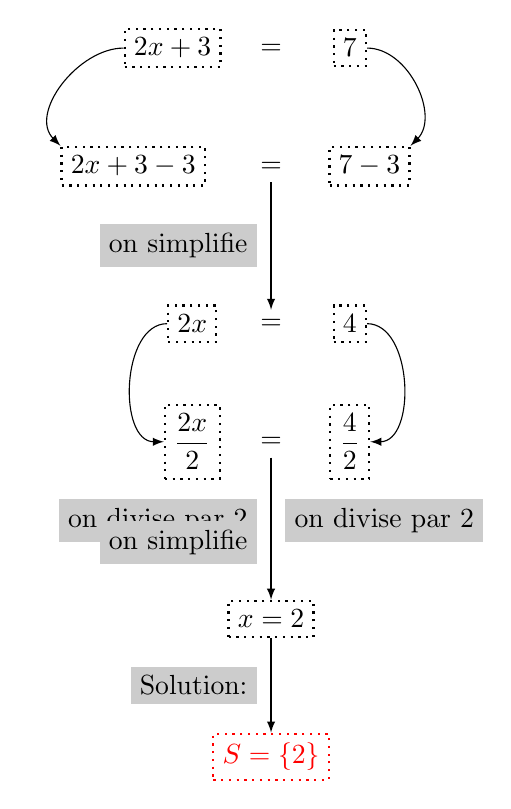
\begin{tikzpicture}
% Styles
 \tikzstyle{membre}= [rectangle,draw,thick,dotted]
 \tikzstyle{operation}=[->,>=latex]
 \tikzstyle{etiquette}=[midway,fill=black!20]
% Equation 1
 \node[membre] (g) at (-1.25,6)  {$2x+3$};
 \node[below=-5pt] at (0,6)  {$=$};
 \node[membre] (d) at (1,6)  {$7$};
% Equation 2
 \node[membre] (gg) at (-1.75,4.5)  {$2x+3-3$};
 \node [below=-5pt] (ee) at (0,4.5)  {$=$};
 \node[membre] (dd) at (1.25,4.5)  {$7-3$};
% Equation 3
 \node[membre] (rg) at (-1,2.5)  {$ 2x$};
 \node [below=-5pt] (rr) at (0,2.5)  {$=$};
 \node[membre] (rd) at (1,2.5)  {$4$};
% Equation 4
 \node[membre] (ggg) at (-1,1)  {$\displaystyle{\frac{2x}{2}}$};
 \node [below=-5pt] (eee) at (0,1)  {$=$};
 \node[membre] (ddd) at (1,1)  {$\displaystyle{\frac{4}{2}}$};
% Equation 5
 \node[membre] (reponse) at (0,-1.25)  {$x=2$};
% solution
 \node[membre,red] (solution) at (0,-3)  {$S=\{2\}$};
 % Fleches et commentaires
 \draw[operation] (g) to[out=180,in=135] (gg.north west)
      node[etiquette,left=5pt]{on soustrait $3$};
 \draw[operation] (d) to[out=0,in=45] (dd.north east)
      node[etiquette,right=5pt]{on soustrait $3$};
 \draw[operation] (ee)--(rr)
      node[etiquette,left=5pt] {on simplifie};
 \draw[operation] (rg) to[out=180,in=180] (ggg)
      node[etiquette,left=5pt]{on divise par $2$};
 \draw[operation] (rd) to[out=0,in=0] (ddd)
      node[etiquette,right=5pt] {on divise par $2$};
 \draw[operation] (eee)--(reponse)
      node[etiquette,left=5pt,pos=0.6] {on simplifie};
 \draw[operation] (reponse)--(solution)
      node[etiquette,left=5pt,midway] {Solution:};
\end{tikzpicture}
\end{center}

\end{document}
